\chapter{State of the Art}
\label{chap:soa}

In this chapter, we introduce the current state of the art in knowledge graph construction using declarative mapping rules. We provide an overview of approaches, techniques and methodologies for constructing and querying (virtual) knowledge graphs based on semantic web technologies. We describe the declarative annotations and mapping languages specifications that have been proposed to construct these kind of data models together with their main features. We also present the current methodologies to evaluate the quality of knowledge graph construction engines such as benchmarkings and test-cases. 

More in detail, in Section \ref{sec:soa_integration} we describe the foundations of data integration concept and its relation with the theoretical contributions where the global schema is defined by an ontology. Section \ref{sec:soa_representation} summarizes the semantic web technologies used for representing and querying data (i.e., the RDF model and the SPARQL query language). Section \ref{sec:soa_annotations} presents an overview of the most important contributions for representing declarative annotations using semantic web technologies, where we are focused on the representations of mapping rules and data constraints. Additionally, Section \ref{sec:soa_engines} presents knowledge graph construction systems and their corresponding optimizations while Section \ref{sec:soa_evaluations} finally, describes the evaluation methodologies for these approaches. We conclude in Section \ref{sec:soa_conclusions} with a set of motivations and gaps that will help to understand the contributions of this thesis.


\section{Data Integration and OBDA}
\label{sec:soa_integration}
A data integration system (DIS) is defined as the process of making available a set of different sources through a common view~\citep{Lenzerini02}. Formally, it is described as $DIS$ = $\langle \mathcal{G}, \mathcal{S}, \mathcal{M} \rangle$, where:
\begin{itemize}
    \item $\mathcal{G}$ is the \textit{global schema}, expressed in a language $\mathcal{L_G}$ over an alphabet $\mathcal{A_G}$.
    
    \item $\mathcal{S}$ is the \textit{source schema}, expressed in a language $\mathcal{L_S}$ over an alphabet $\mathcal{A_S}$.
    
    \item $\mathcal{M}$ is the \textit{mapping} between $\mathcal{G}$ and $\mathcal{S}$, constituted by a set of assertions matching queries over $\mathcal{S}$ and $\mathcal{G}$, in order to establish correspondences between concepts in both schemes.
\end{itemize}

Different types of data integration systems have been proposed. Data warehouses~\citep{vassiliadis2009survey} are proposed to integrate multiple and heterogeneous data sources in a centralized place, which is usually known in enterprises ecosystems as an \textit{extract-transform-load} process (ETL). In contrast, mediators~\citep{wiederhold1992mediators} have been proposed as another data integration approach where the data remains in the data sources. For accessing the data, queries defined over the global schema are translated to the source schema and executed. There are multiple systems that implement these ideas with their corresponding optimizations~\citep{tsimmis1994,rajaraman1996querying,roth1997don}.

Ontology based data access (OBDA) and integration (OBDI) are data integration systems where the global schema is defined by an ontology~\citep{poggi2008linking}. The formal framework presented in~\citep{xiao2018obdasurvey} defines an OBDA specification as a tuple $P$ = $\langle O,S,M\rangle$ where $O$ is an ontology, $S$ is the source schema, and $M$ a set of mappings. Additionally, an OBDA instance is defined as a tuple $PI$ = $\langle P,D\rangle$ where P is an OBDA specification and $D$ is a data instance conforming to $S$. The main difference between OBDA and OBDI systems is that in OBDA $D$ is fixed to an specific data format, while OBDI extends $D$ to cover heterogeneous data sources and formats. In both ontology-based approaches, two different alternatives exist to enable data access: (1) those where data are materialized taking into account the mappings and the ontologies which can be seen as a ontology-based ETL process, and (2) those where the transformation is done on the queries, which can then be evaluated on the original data sources, so, it can be defined as a new kind of mediator system. In this work we refer to the first alternative as   a materialized knowledge graph construction process, while the second alternative is defined as a virtual knowledge graph construction one. As we are focused on creating KG from heterogeneous data sources, both alternatives can be described as an OBDI approach.

\section{Representation and Query Language for the Semantic Web}
\label{sec:soa_representation}
\subsection{RDF: Resource Description Framework}

\subsection{SPARQL}




\section{Annotations in Knowledge Graph Construction}
\label{sec:soa_annotations}
One of the main components for the construction of knowledge graphs are the annotations. Additionally to the mapping rules, that relate the target model with the input sources in a typical data integration system definition, we include in the annotations set the constraints concept. In a DIS, the constrains property allows to: i) define ad-hoc transformation functions that permit the cleaning and preparation of the input data; ii) definition of metadata annotations to describe the content of the input source. This property is essential during a knowledge graph construction process as it is able to deal with the typical features of heterogeneous data sources such as the absence of a well-defined and fixed data schema, a normalized database instance or the non-explicit declarations of relations among the sources. We start this section discussing existing approaches for the design of mappings. Then, we describe the current mapping language specifications and their standardization through the W3C. Finally, we present approaches to define, declaratively, constraints over a DIS.

\subsection{Mapping Rules}
The mapping layer contains information about how the input sources are related with the target model. There are two basic approaches for defining mapping rules in a data integration system: Local as a View (LAV) and Global as a View (GAV). In semantic web, the usual followed approach to define this rules is the Global as View one. We now provide a description of each proposals more in detail.

\subsubsection{Local as a View Mapping rules (LAV)}
In \citep{ullman1997information} the elements of the source schema $S$ are mapped  to a query $Q_G$ over the target schema $G$. The main benefits of this approach is that it supports continuous changes of the source schema (e.g., adding new sources or modify their underlying representation) since there is no need to change the query processing component. Thus, LAV is usually useful when the global schema $G$ is stable but the local schema $S$ may suffer modifications over the time. However, one of its main disadvantages is that cannot represent source $S$ information if it is not modeled in the global schema, hence, the approach usually provides partial answers for a query $Q_G$. Query translation following this approach is not a trivial process, as the $Q_G$ has to be translated to an equivalent query over the source schema $S$. These techniques are usually known as query translation using views~\citep{halevy2001answering}.

ToDo: ADD EXAMPLE

\subsubsection{Global as a View Mapping Rules (GAV)}
Global as view are defined in \citep{halevy2001answering}, where each element of the global schema $G$ is mapped to a query over $Q_S$ the source schema $S$. Opposed to LAV approach, the benefits of following a GAV approach is that it supports changes over the global schema $G$, as the queries are defined following the source schema $S$. Although there are no theoretical limitations to provide access to other data formats, ontology-based data integration processes have been traditionally focused on allowing the integration of relational databases as source schema, based on SPARQL-to-SQL translation techniques. Due to the aforementioned limitations in these techniques for LAV approaches, most of the semantic web mapping rules specifications following the GAV approach (e.g., R$_2$O, DR2Q, R2RML). 

ToDO: ADD EXAMPLE

\subsubsection{R2RML: W3C Recommendation}
Since 2012, R2RML is a W3C recommendation to declarative declare mapping rules between RDF and RDB~\citep{R2RML}. These rules are defined in an R2RML mapping document, which is formed by a set of Triples Maps (\texttt{rr:TriplesMap}). Usually, each Triple Map defines the rules for generating the entities and their properties of a defined class in the ontology and are defined as:
\begin{itemize}
    \item one logical table (\texttt{rr:LogicalTable}) that specifies the source relational table/view
    \item one subject map (\texttt{rr:SubjectMap}) that specifies how to generate the subjects of the triples and the corresponding class.
    \item from zero to multiple predicate-object maps (\texttt{rr:PredicateObjectMap}). Predicate-object map is formed by one or many predicate maps (\texttt{rr:PredicateMap}), and one to many object maps (\texttt{rr:ObjectMap}) or reference-object maps (\texttt{rr:RefObjectMap}). This last one is used when joins among logical sources are defined.
\end{itemize}

\begin{figure}[!h]
\centering
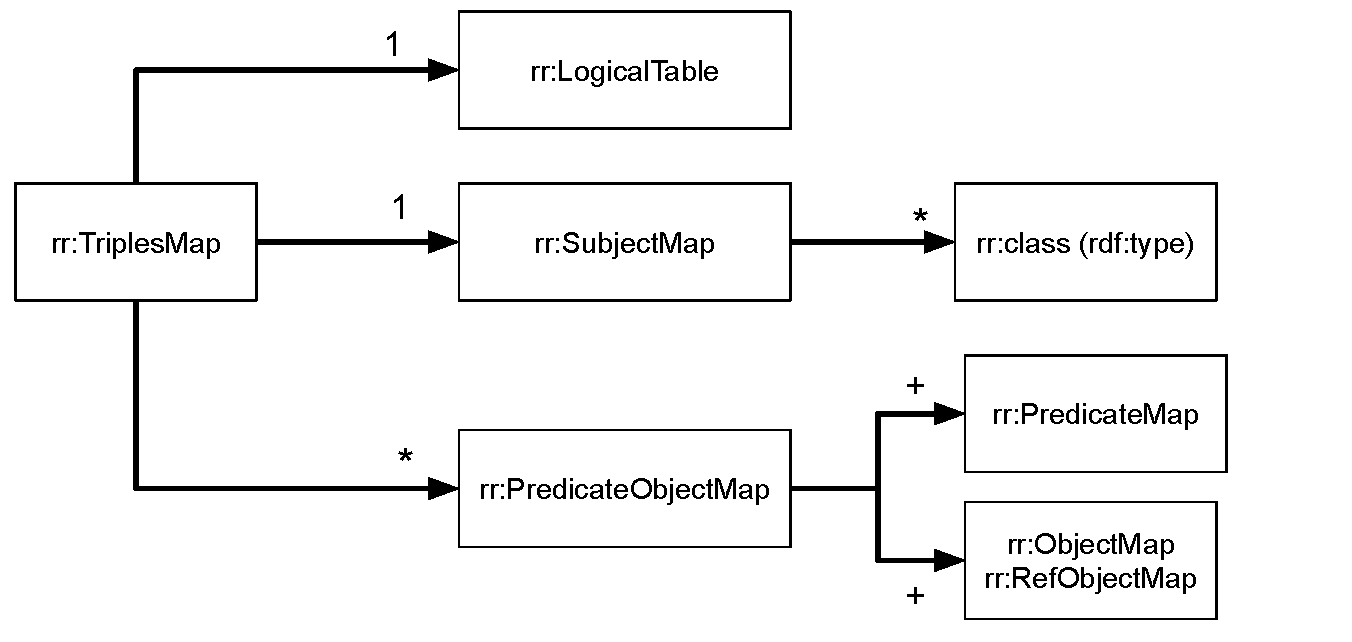
\includegraphics[width=\textwidth]{figures/state-of-the-art/R2RML-structure.pdf}
\caption{R2RML structure with its relevant properties}
\label{fig:soa_r2rml-structure}
\end{figure}

Figure \ref{fig:soa_r2rml-structure} shows the basic structure of an R2RML Triples Map, with the relations between its main properties and their cardinalities. \texttt{rr:SubjectMap}, \texttt{rr:PredicateMap} and \texttt{rr:ObjectMap} are defined as term maps (\texttt{rr:TerMap}. This property is used to generate the desirable RDF terms, either as IRIs (\texttt{rr:IRI}) Blank Nodes (\texttt{rr:BlankNode}) or literal (\texttt{rr:Literal}). The values of the term maps can be specify using the following properties: \texttt{rr:Constant} for constant values, \texttt{rr:Column} for values obtained directly from a column of a table or \texttt{rr:Template} for the ones that are a concatenation between a string and a column reference, for example, to generate subject IRIs. Furthermore, additional information can be provided such as the language of a literal, using the \texttt{rr:Language} property, or its corresponding datatype with \texttt{rr:Datatype}. Figure \ref{fig:soa_termmap-structure} gives an overview of the R2RML term map.


\begin{figure}[!h]
\centering
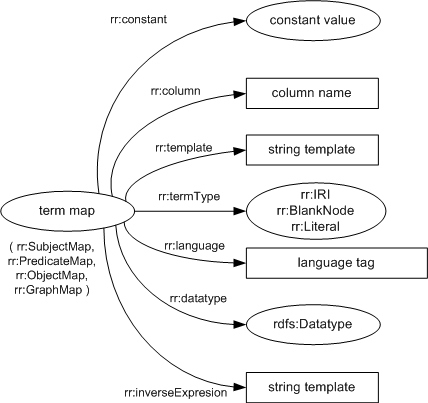
\includegraphics[width=0.7\textwidth]{figures/state-of-the-art/term-map.png}
\caption{R2RML \texttt{rr:TermMap} overview}
\label{fig:soa_termmap-structure}
\end{figure}

We provide a complete example of the construction of a knowledge graph through an R2RML mapping. The input table (Figure \ref{fig:soa_csv}) represents information about the stop times for a giving trip of the Madrid's metro system. It provides the corresponding identifier for the trip and each stop together with the pickup time and type. Figure \ref{fig:soa_r2rml} shows the R2RML mapping for transforming the input table to a RDF dataset following the LinkedGTFS\footnote{\url{https://lov.linkeddata.es/dataset/lov/vocabs/gtfs}} ontology. We can observe that the subject map uses a \texttt{rr:template} with reference to three different columns of the table to generate unique identifiers for the IRIs. The set of \texttt{rr:PredicateObjectMap} (POM) defines the rules to generate three different properties of the \texttt{gtfs:StopTime} class. The \texttt{gtfs:arrivalTime} POM uses the \texttt{rr:dataType} property to declare the type of the input data, \texttt{gtfs:pickupType} uses the \texttt{rr:template} to generate an uri-based literal in the output dataset, and finally, \texttt{gtfs:trip} predicate has a \texttt{rr:RefObjectMap} to generate its corresponding object, referencing to the corresponding IRI trip defined in antoher TriplesMap. Finally, the output RDF dataset is shown in Figure \ref{fig:soa_rdf}.

\begin{figure}[!h]
\centering
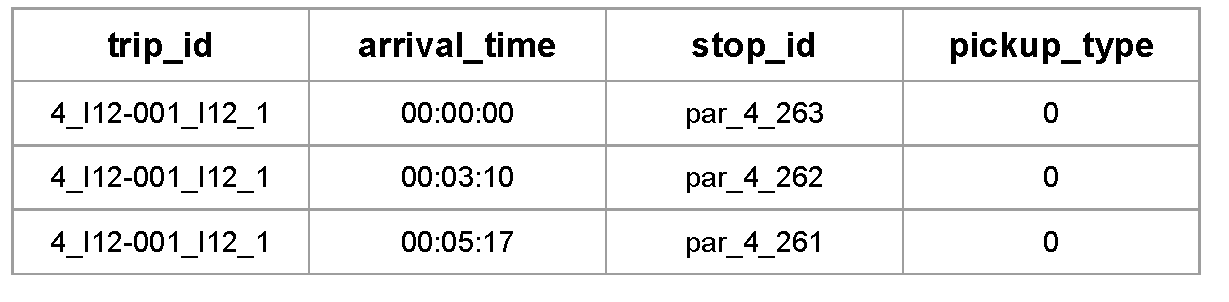
\includegraphics[width=0.85\textwidth]{figures/state-of-the-art/Stop_times CSV.pdf}
\caption{Excerpt of a Stop-times table}
\label{fig:soa_csv}
\end{figure}

\begin{figure}[!h]
\centering
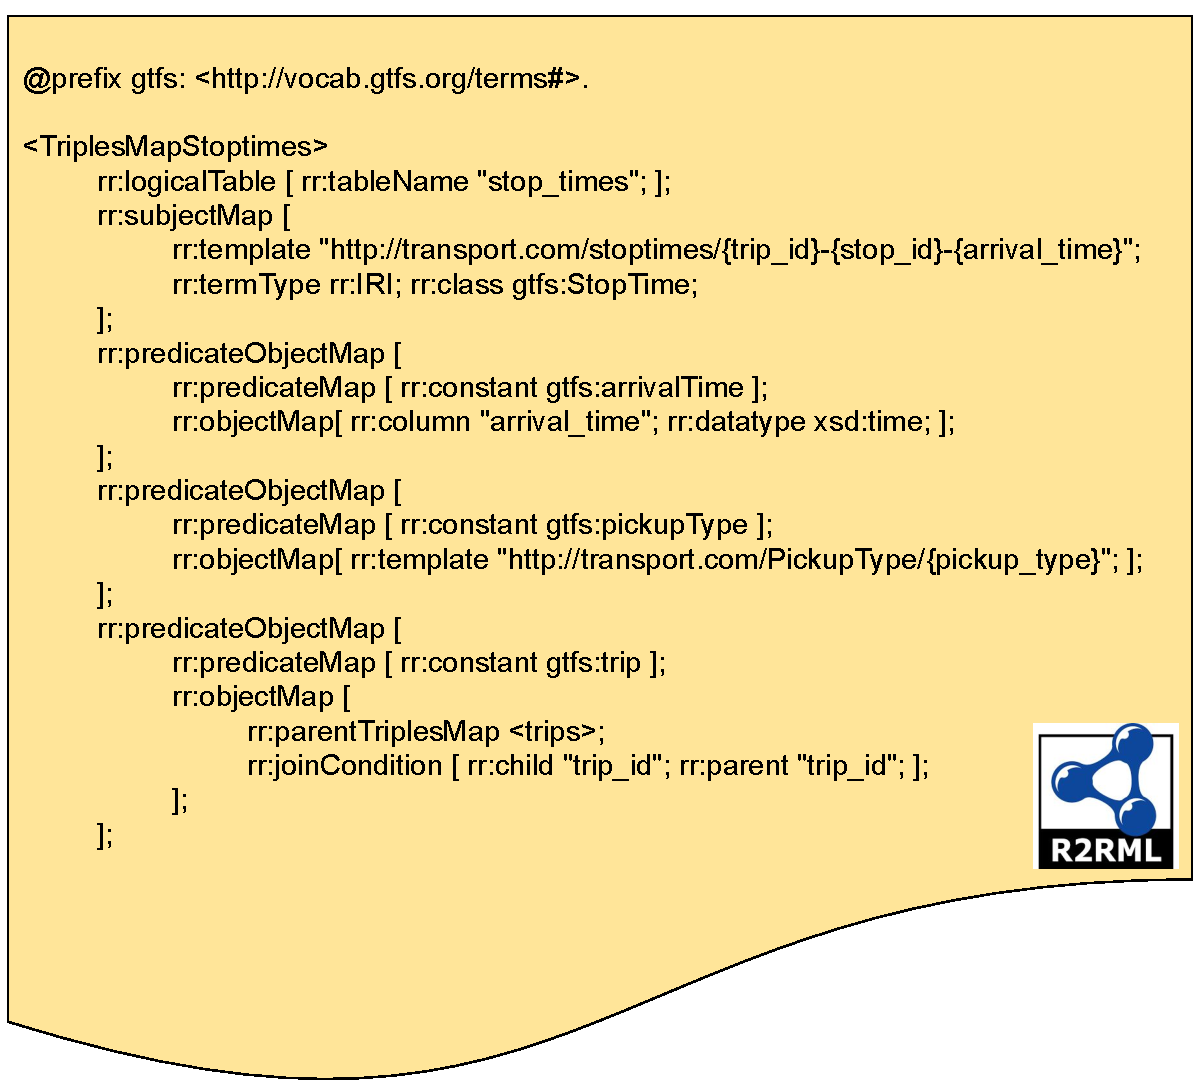
\includegraphics[width=0.85\textwidth]{figures/state-of-the-art/R2RML-example.pdf}
\caption{R2RML mapping for stop-times table}
\label{fig:soa_r2rml}
\end{figure}


\begin{figure}[!h]
\centering
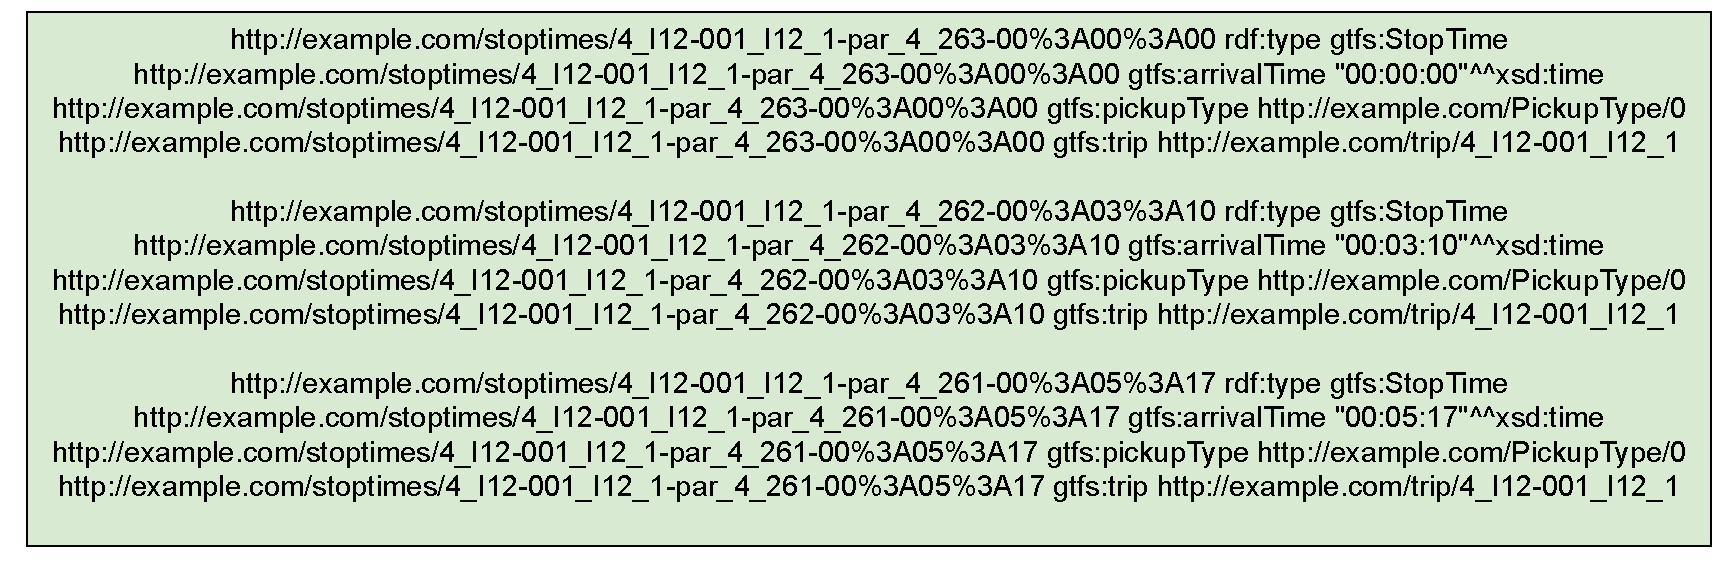
\includegraphics[width=0.85\textwidth]{figures/state-of-the-art/RDF from Stop_times.pdf}
\caption{Output RDF dataset after parsing the R2RML document}
\label{fig:soa_rdf}
\end{figure}



\subsubsection{RML: Extending R2RML for Heterogeneous Data}
The RDF Mapping Language (RML)~\citep{dimou2014rml} proposes to extend the R2RML mapping specification to cover other kinds of data formats such as CSV, XML or JSON, hence, this specification is one of the most used for constructing knowledge graph from heterogeneous data sources. In this section we first explain the main differences between RML and R2RML and then we describe other mapping specifications or approaches that are able to construct KGs from heterogeneous data sources.


\begin{table}[h]
\centering
\caption{The differences between R2RML and RML}
\label{tab:soa_rmlvsr2rml}
\begin{tabular}{l|c|c}
                                          & \textbf{R2RML}                      & \textbf{RML}                         \\
\hline                                          
\textbf{Input reference}                  & Logical Table                       & Logical Source                       \\
\hline
\textbf{Data source language}             & SQL (implicit)                      & Reference Formulation (explicit)     \\
\hline
\multirow{2}{*}{\textbf{Value reference}} & \multirow{2}{*}{column}             & Logical reference \\
                                          &                                     & (valid expression acc. \\
                                          &                                     & Reference Formulation) \\
\hline                                          
\multirow{2}{*}{\textbf{Iteration}}       & \multirow{2}{*}{per row (implicit)} & per record        \\
                                          &                                     & (explicit -- valid expression        \\
                                          &                                     & acc. Reference Formulation)
\end{tabular}
\end{table}


\noindent Summarized in Table \ref{tab:soa_rmlvsr2rml}, the main differences between R2RML and RML are:

\noindent\textbf{{Logical Source.}} A Logical Source extends R2RML's Logical Table and describes the input data source used to generate the RDF. The Logical Table is only able to describe relational databases,whereas the Logical Source defines different heterogeneous data sources, including relational databases.

\noindent\textbf{{Reference Formulation}} As RML is designed to support heterogeneous data sources, data sources in different formats needs to be supported. One refers to data in a specific format according to the grammar of a certain formulation, which might be path and query languages or custom grammars. For example, one can refer to data in an XML file via XPath and in a relational database via SQL. To this end, the \emph{Reference Formulation} was introduced indicating the formulation used to refer to data in a certain data source.

\noindent\textbf{{Iterator}} In R2RML it is specified that processors iterate over each row to generate RDF. However, as RML is designed to support heterogeneous data sources, the iteration pattern cannot always be implicitly assumed. For example, iterating over a specific set of objects is done by selecting them via a JSONPath expression. To this end, the \emph{Iterator} was introduced which determines the iteration pattern over the data source and specifies the extract of data used to generate RDF during each iteration. The iterator is not required to be specified if there is no need to iterate over the input data.

\noindent\textbf{{Logical Reference}} When referring to values in a table or view of a relational database, R2RML relies on column names. However, as RML is designed to support heterogeneous data sources, rules may also refer to elements and objects, such as in the case of XML and JSON. Consequently, references to values should be valid with respect to the used reference formulation. For example, a reference to an attribute of a JSON object should be a valid JSONPath expression. To this end, (i) the \verb|rml:reference| is introduced to replace \verb|rr:column|, (ii) when a template is used, via \verb|rr:template|, the values between the curly brackets should have an expression that is valid with respect to the used reference formulation, and (iii) \verb|rr:parent| and \verb|rr:child| of a Join Condition should also have an expression that is valid with respect to the used reference formulation.

\subsection{Declarative Constraints: Transformation Functions and Metadata}
Data constraints play a key role during a data integration process~\citep{cali2002data}. This property allows to validate an input dataset $D$ against an schema $S$. In previous proposals of knowledge graph construction over relational database (OBDA), they assume the existence of integrity constraints explicitly defined over the schema $S$ to propose their optimizations in SPARQL-to-SQL processes. Additionally, mapping recommendations (i.e., R2RML) for RDB2RDF approaches declare that cleaning or preparation steps are not part of the KG construction process and they have to be performed before running it. However, during the construction of a KG from heterogeneous data sources, these data may not be normalized, and information about relationships or column/key names are not always descriptive or homogeneous, among other possible issues. Hence, data consumers are usually forced to apply ad-hoc or manual data wrangling processes to consume these kind of data. In order to try to avoid manual and not reproducible cleaning/preparation steps, there are a set of declarative proposals to allow the description of constraints over data on the web. Specifically, we will be focused on two different ways to declare constraints: extensions of mapping specifications for include the possibility to define transformation functions inside the mapping rules and metadata to describe data content on the web. 

\subsubsection{Transformation Functions in Mappings}
Rahm and Do~\citep{rahm2000data} have reported the relevance of data transformations expressed with functions during data curation and integration. Grounding on this statement, different approaches have been proposed for facilitating the definition of functions to enhance data curation (e.g., \citep{galhardas2001declarative,GuptaSKGTM12,raman2001potter}). Similarly, declarative languages have been proposed to allow for the definition of functions in the mappings. An approach independent of a specific implementation context is described in~\citep{demeester2019implementation}. It enables the description, publication and exploration of functions and instantiation of associated implementations. The proposed model is the so called Function Ontology~\citep{de2016ontology} and the publication method follows the Linked Data principles. It is used as an extension over RML mapping rules to declarative allow the declaration of these transformation functions~\citep{de2017declarative}. Previous works related to this topic focus on developing ad-hoc and programmed functions. For example, R2RML-F~\citep{debruyne2016r2rml} and FunUL~\cite{junior2016funul,junior2016incorporating} allow using functions in the value of the \texttt{rr:objectMap} property, so as to modify the value of the table columns from a relational database first (R2RML-F) and other kinds of formats after (FunUL). KR2RML~\citep{slepicka2015kr2rml}, used in Karma, extends R2RML by adding transformation functions in order to deal with nested values. OpenRefine enables such transformations with the usage of GREL functions, which can be used in its RDF extension. 

ToDo: add FnO examples

\subsubsection{Metadata for data on the web}


\section{Knowledge Graph Construction Engines}
\label{sec:soa_engines}

\section{Evaluation of Knowledge Graph Construction}
\label{sec:soa_evaluations}

\subsection{Test-Cases}
\subsection{Benchmarks}



\section{Conclusions}
\label{sec:soa_conclusions}
